\section{Modellierung der Daten}
\subsection{Darstellung der Klassen}
In diesem Kapitel geht es um die objektorientierte Analyse der in dem letzten Kapitel spezifizierten Anforderungen. Ziel ist es mit Hilfe eines Klassendiagramms die Daten des System visuell darzustellen und die Beziehungen der Klassen untereinander zu modellieren. Diese Klasendiagramme sollen einen tatsächlichen Aufbau des Systems darstellen, der in einem späteren, nicht im Rahmen dieser Arbeit angefertigten, Entwurf und Implementierung als Vorlage dienen soll, um die tatsächlichen Klassen aufzubauen. Da dieses Klassendiagramm bereits in der Konzeptionsphase des Systems aufgebaut wird, haben diese Modellierungen keinen Anspruch auf Richtigkeit, da aus technischen oder organisatorischen Gründen zu einem späteren Zeitpunkt noch Änderungen erfolgen können. Diese Änderungen können zum Beispiel aufgrund von technischen Restriktionen der Entwicklungsumgebung oder aufgrund von Wünschen des Auftraggebers auftreten.
\\Um die Übersichtlichkeit zu bewahren wird als erstes ein Übersichtsklassendiagramm gezeigt, dass die Klassen nur bei ihrem Namen nennt und die Beziehung zwischen den Klassen darstellt. Im Anschluss erfolgt die Beschreibung der Klassen und den herrschenden Assoziationen, Aggregationen, Kompositionen und Generalisierungen. Im Anschluss erfolgt die vollständige Darstellung der Klassen in einem erweiterten Klassendiagramm, indem zusätzlich die Operationen und Attribute dargestellt sind. Danach werden die Attribute und Operationen exemplarisch anhand von drei ausgewählten Klassen spezifiziert. Zum Ende dieses Kapitels erfolgt die Zusammenfassung der Klassen in einem Paketdiagramm.    

\newpage
\subsection{Übersichtsklassendiagramm}
\begin{figure}[h!]
    \centering
    \includegraphics[scale=0.6]{./Bilder/Übersichtsklassendiagramm.png}
    \caption[Übersichtsklassendiagramm]{Übersichtsklassendiagramm}
    \label{fig:Übersichtsklassendiagramm}
\end{figure}
\emph{Zur verbesserten Anschauung ist das Diagramm ebenfalls im Verzeichnis ./Bilder/Übersichtsklassendiagramm.png dieser Arbeit abgelegt.}

\newpage
\subsection{Klassen und Beziehungen}
\subsubsection{Beschreibung der Klassen}
In den nachfolgenden Tabelle werden zuerst die ermittelten Klassen beschrieben, danach die Beziehungen mit Assoziationen und die Beziehungen mit Generalisierungen.

\begin{xltabular}{\textwidth}{|p{0.3\textwidth}|p{0.642\textwidth}|}
    \hline
    \textbf{Klasse} & \textbf{Beschreibung} \\\hline\hline
    Benutzer & Eine natürliche Person, die ein Benutzerkonto im System hat.\\\hline
    Administrator & Eine natürliche Person, die für die Verwaltung des Systems zuständig ist. \\\hline
    Projektleiter & Eine natürliche Person, die ein S/4HANA-Transformationsprojekt leitet. \\\hline
    Teilprojektleiter & Eine natürliche Person, die ein Teilprojekt in einem S/4HANA-Transformationsprojekt leitet. \\\hline
    Projektmitarbeiter & Eine natürliche Person, die Mitarbeiter in einem S/4HANA-Transformationsprojekt ist. \\\hline
    Kunde &  Eine natürliche Person, die Kunde eines S/4HANA-Transformationsprojekt ist.\\\hline
    Projekt & Eine Einheit, die ein S/4HANA-Transformationsprojekt abbildet. \\\hline
    Teilprojekt & Eine Einheit, die ein Teilprojekt in einem S/4HANA-Transformationsprojekt abbildet. \\\hline
    Projektphase & Ein Zeitraum in einem S/4HANA-Transformationsprojekt\\\hline
    Kriterium & Eine Eigenschaft einer Projektphase, die während der S/4HANA-Transformation erfüllt wird. \\\hline
    BoolschesKriterium & Ein Kriterium, das einen Ja- oder Nein-Wert speichert.\\\hline
    Textkriterium & Ein Kriterium, das eine Zeichenkette speichert.\\\hline
    Zahlenkriterium & Ein Kriterium, das eine Ganzzahl oder Gleitkommazahl speichert. \\\hline
    Prozess &  Ein in SAP abgebildetete Folge von Aktivitäten.\\\hline
    Subprozess &  Ein in sich geschlossener Abschnitt eines Prozess.\\\hline
    Prozessschritt & Eine Aktivität eines Prozess.\\\hline
\end{xltabular}
\captionof{table}[Klassenbeschreibungen]{Beschreibung der ermittelten Klassen}

\subsubsection{Beschreibung der Assoziationen}
Assoziationen sind Beziehungen, die zwischen Klassen bestehen und können unterschiedlicher Natur sein. Assoziationen sind bidirektional und funktionieren deswegen in beide Richtungen.\\
\begin{xltabular}{\textwidth}{|p{0.3\textwidth}|p{0.145\textwidth}|p{0.145\textwidth}|p{0.3\textwidth}|}
    \hline
    \multicolumn{4}{|c|}{\textbf{Klassen mit Assoziationen}}\\\hline\hline
    %%%%%%
    Administrator & 1 & 0..* & Projekt\\\hline
    \multicolumn{4}{|p{0.942\textwidth}|}{Ein Administrator kann kein, oder mehrere Projekte im System erstellen, aber ein Projekt kann nur von genau einem Administrator erstellt werden.}\\\hline\hline
    %%%%%%
    %%%%%%
    Benutzer & 1..* & 0..* & Projekt\\\hline
    \multicolumn{4}{|p{0.942\textwidth}|}{Ein Benutzer kann kein, oder mehreren Projekten im System zugeordnet sein und ein Projekt kann keinem oder mehreren Benutzer zugeordnet werden.}\\\hline\hline
    %%%%%%
    %%%%%%
    Administrator & 1..* & 0..* & Benutzer\\\hline
    \multicolumn{4}{|p{0.942\textwidth}|}{Ein Administrator kann ein keinen oder mehrere Benutzer verwalten und ein Benutzer kann von einem oder mehreren Administratoren verwaltet werden.}\\\hline\hline
    %%%%%%
    Projektleiter & 1..* & 1 & Projektphase\\\hline
    \multicolumn{4}{|p{0.942\textwidth}|}{Ein Projektleiter kann eine oder mehrere Projektphasen erstellen aber eine Projektphase kann nur durch genau einen Projektleiter erstellt werden.}\\\hline\hline
    %%%%%%
    %%%%%%
    Teilprojektleiter & 1 & 0..* & Kriterium\\\hline
    \multicolumn{4}{|p{0.942\textwidth}|}{Ein Teilprojektleiter kann kein, oder belieb viele Kriterien erstellen, ein Kriterium wird jedoch nur durch eine Teilprojektleiter erstellt.}\\\hline\hline
    %%%%%%
    Projektleiter & 1..* & 0..* & Projekt\\\hline
    \multicolumn{4}{|p{0.942\textwidth}|}{Ein Projektleiter verwaltet kein oder mehrere Projekte und ein Projekt wird durch mindestens einen Projektleiter verwaltet}\\\hline\hline
    %%%%%%
    Teilprojektleiter & 1..* & 0..* & Teilprojekt\\\hline
    \multicolumn{4}{|p{0.942\textwidth}|}{Ein Teilprojektleiter verwaltet kein oder mehrere Teilprojekte und ein Teilprojekt wird durch mindestens einen Projektleiter verwaltet}\\\hline\hline
    %%%%%%
    Projektmitarbeiter & 1 & 0..* & Kriterium\\\hline
    \multicolumn{4}{|p{0.942\textwidth}|}{Ein Projektmitarbeiter kann kein, oder belieb viele Kriterien erstellen, ein Kriterium wird jedoch nur durch einen Projektmitarbeiter erstellt.}\\\hline\hline
    Prozessschritt & 0..* & 0..* & Kriterium\\\hline
    \multicolumn{4}{|p{0.942\textwidth}|}{Ein Prozessschritt prägt kein, oder beliebig viele Kriterien aus und ein Kriterium wird durch kein oder beliebig vielen Prozessschritten ausgeprägt.}\\\hline\hline
    Kunde & 0..* & 0..1 & Projekt\\\hline
    \multicolumn{4}{|p{0.942\textwidth}|}{Ein Kunde betrachtet keins oder ein Projekt und ein Projekt wird von keinem oder mehreren Kunden betrachtet.}\\\hline\hline
    Subprozess & 0..1 & 1..* & Prozessschritt\\\hline
    \multicolumn{4}{|p{0.942\textwidth}|}{Ein Subprozess beinhaltet einen oder mehrere Prozessschritte und ein Prozessschritt kann zu keinem oder einem Prozessschritt gehören, da Subprozesse nur optional sind.}\\\hline
    
\end{xltabular}
\captionof{table}[Klassen mit Assoziationen]{Beschreibung der ermittelten Klassen mit Assoziationen}

\newpage
\subsubsection{Beschreibung der Aggregationen}
Aggregationen sind eine besondere Form von Assoziationen, bei denen Objekte einer Klasse einen Teil von einer anderen Klasse darstellen. Dadurch ist es möglich beispielsweise Besitz darzustellen.\\

\begin{xltabular}{\textwidth}{|p{0.3\textwidth}|p{0.145\textwidth}|p{0.145\textwidth}|p{0.3\textwidth}|}
    \hline
    \multicolumn{4}{|c|}{\textbf{Klassen mit Aggregationen}}\\\hline\hline
    Teilprojekt & 1..* & 0..* & Prozess\\\hline
    \multicolumn{4}{|p{0.942\textwidth}|}{Ein Teilprojekt beinhaltet keinen oder mehrere Prozesse, ein Prozess gehört aber immer zu einem oder mehreren Teilprojekten. Ein Teilprojekt ohne Prozesse kann existieren, ein Prozess ohne nicht mindestens ein Teilprojekt jedoch nicht.}\\\hline\hline
    Teilprojekt & 1 & 0..1 & Projektmitarbeiter\\\hline
    \multicolumn{4}{|p{0.942\textwidth}|}{Ein Teilprojekt hat keinen oder mehrere zugeordnete Projektmitarbeiter und ein Projektmitarbeiter ist immer einem Teilprojekt zugeordnet. Ein Teilprojekt ohne Projekmitarbeiter kann existieren, ein Projektmitarbeiter ohne Teilprojekt jedoch nicht.}\\\hline\hline
    Prozess & 1 & 0..* & Subprozess\\\hline
    \multicolumn{4}{|p{0.942\textwidth}|}{Ein Prozess kann keine oder mehrere Subprozesse beinhalten, ein Subprozess gehört immer zu genau einem Prozess. Ein Prozess ohne Subprozesse kann existieren, ein Subprozess ohne Prozess jedoch nicht.}\\\hline
\end{xltabular}
\captionof{table}[Klassen mit Aggregation]{Beschreibung der ermittelten Klassen mit Aggregationen}
\newpage
\subsubsection{Beschreibung der Kompositionen}
Kompositionen sind eine besondere Form von Aggregation, bei denen die Objekte der einen Klasse nicht ohne die Objekte der anderen Klasse existieren können.\\

\begin{xltabular}{\textwidth}{|p{0.3\textwidth}|p{0.145\textwidth}|p{0.145\textwidth}|p{0.3\textwidth}|}
    \hline
    \multicolumn{4}{|c|}{\textbf{Klassen mit Kompositionen}}\\\hline\hline
    Projekt & 1 & 1..5 & Projektphase\\\hline
    \multicolumn{4}{|p{0.942\textwidth}|}{Ein Projekt kann eine oder bis zu fünf Projektphasen beinhalten und eine Projektphase gehört immer zu genau einem Projekt. Ein Projekt ohne Projektphasen kann nicht existieren, eine Projektphase ohne Projekt ebenfalls nicht.}\\\hline\hline
    %%%%%%
    Projekt & 1 & 1..* & Teilprojekt\\\hline
    \multicolumn{4}{|p{0.942\textwidth}|}{Ein Projekt kann ein oder mehrere Teilprojekte beinhalten und ein Teilprojekt gehört zu genau einem Projekt. Ein Projekt ohne Teilprojekte kann nicht existieren, ein Teilprojekt ohne Projekt ebenfalls nicht.}\\\hline\hline
    %%%%%%
    Projektphase & 1 & 1..* & Kriterium\\\hline
    \multicolumn{4}{|p{0.942\textwidth}|}{Eine Projektphase hat ein oder mehrere Kriterien und ein Kriterium gehört zu genau einer Projektphase. Eine Projektphase ohne Kriterien kann nicht existieren, ein Kriterium ohne Projektphase ebenfalls nicht.}\\\hline\hline
    %%%%%%
    Prozess & 1 & 1..* & Prozessschritt\\\hline
    \multicolumn{4}{|p{0.942\textwidth}|}{Ein Prozess hat ein oder mehrere Prozessschritte und ein Prozessschritt gehört immer zu genau einem Prozess. Ein Prozess ohne Prozessschritte kann nicht existieren, ein Prozessschritt ohne Prozess ebenfalls nicht.}\\\hline
    %%%%%%
\end{xltabular}
\captionof{table}[Klassen mit Kompositionen]{Beschreibung der ermittelten Klassen mit Kompositionen}
\newpage
\subsubsection{Beschreibung der Generalisierungen}
Generalisierungen sind Vererbungsbeziehungen, bei denen es eine Basisklasse gibt, die ihre Kriterien an eine oder mehrere spezialisierte, bzw. abgeleitete Klassen vererbt.\\

\begin{xltabular}{\textwidth}{|p{0.472\textwidth}|p{0.472\textwidth}|}
    \hline
    \multicolumn{2}{|c|}{\textbf{Klassen mit Generalisierungen}}\\\hline\hline
    BoolschesKriterium, Textkriterium, Zahlenkriterium & Kriterium \\\hline
    \multicolumn{2}{|p{0.944\textwidth}|}{Die Klasse Kriterium ist abstrakt und vererbt ihre Eigenschaften an die abgeleiteten Klassen BoolschesKriterium, Textkriterium und Zahlenkriterium.}\\\hline\hline
    Administrator, Projektleiter, Teilprojektleiter, Projektmitarbeiter, Kunde & Benutzer \\\hline
    \multicolumn{2}{|p{0.944\textwidth}|}{Die Klasse Benutzer ist abstrakt und vererbt ihre Eigenschaften an die abgeleiteten Klassen Administrator, Projektleiter, Teilprojektleiter, Projektmitarbeiter und Kunde.}\\\hline
\end{xltabular}
\captionof{table}[Klassen mit Generalisierungen]{Beschreibung der ermittelten Klassen mit Generalisierungen}
\newpage
\subsection{Erweitertes Klassendiagramm}
\begin{figure}[h!]
    \centering
    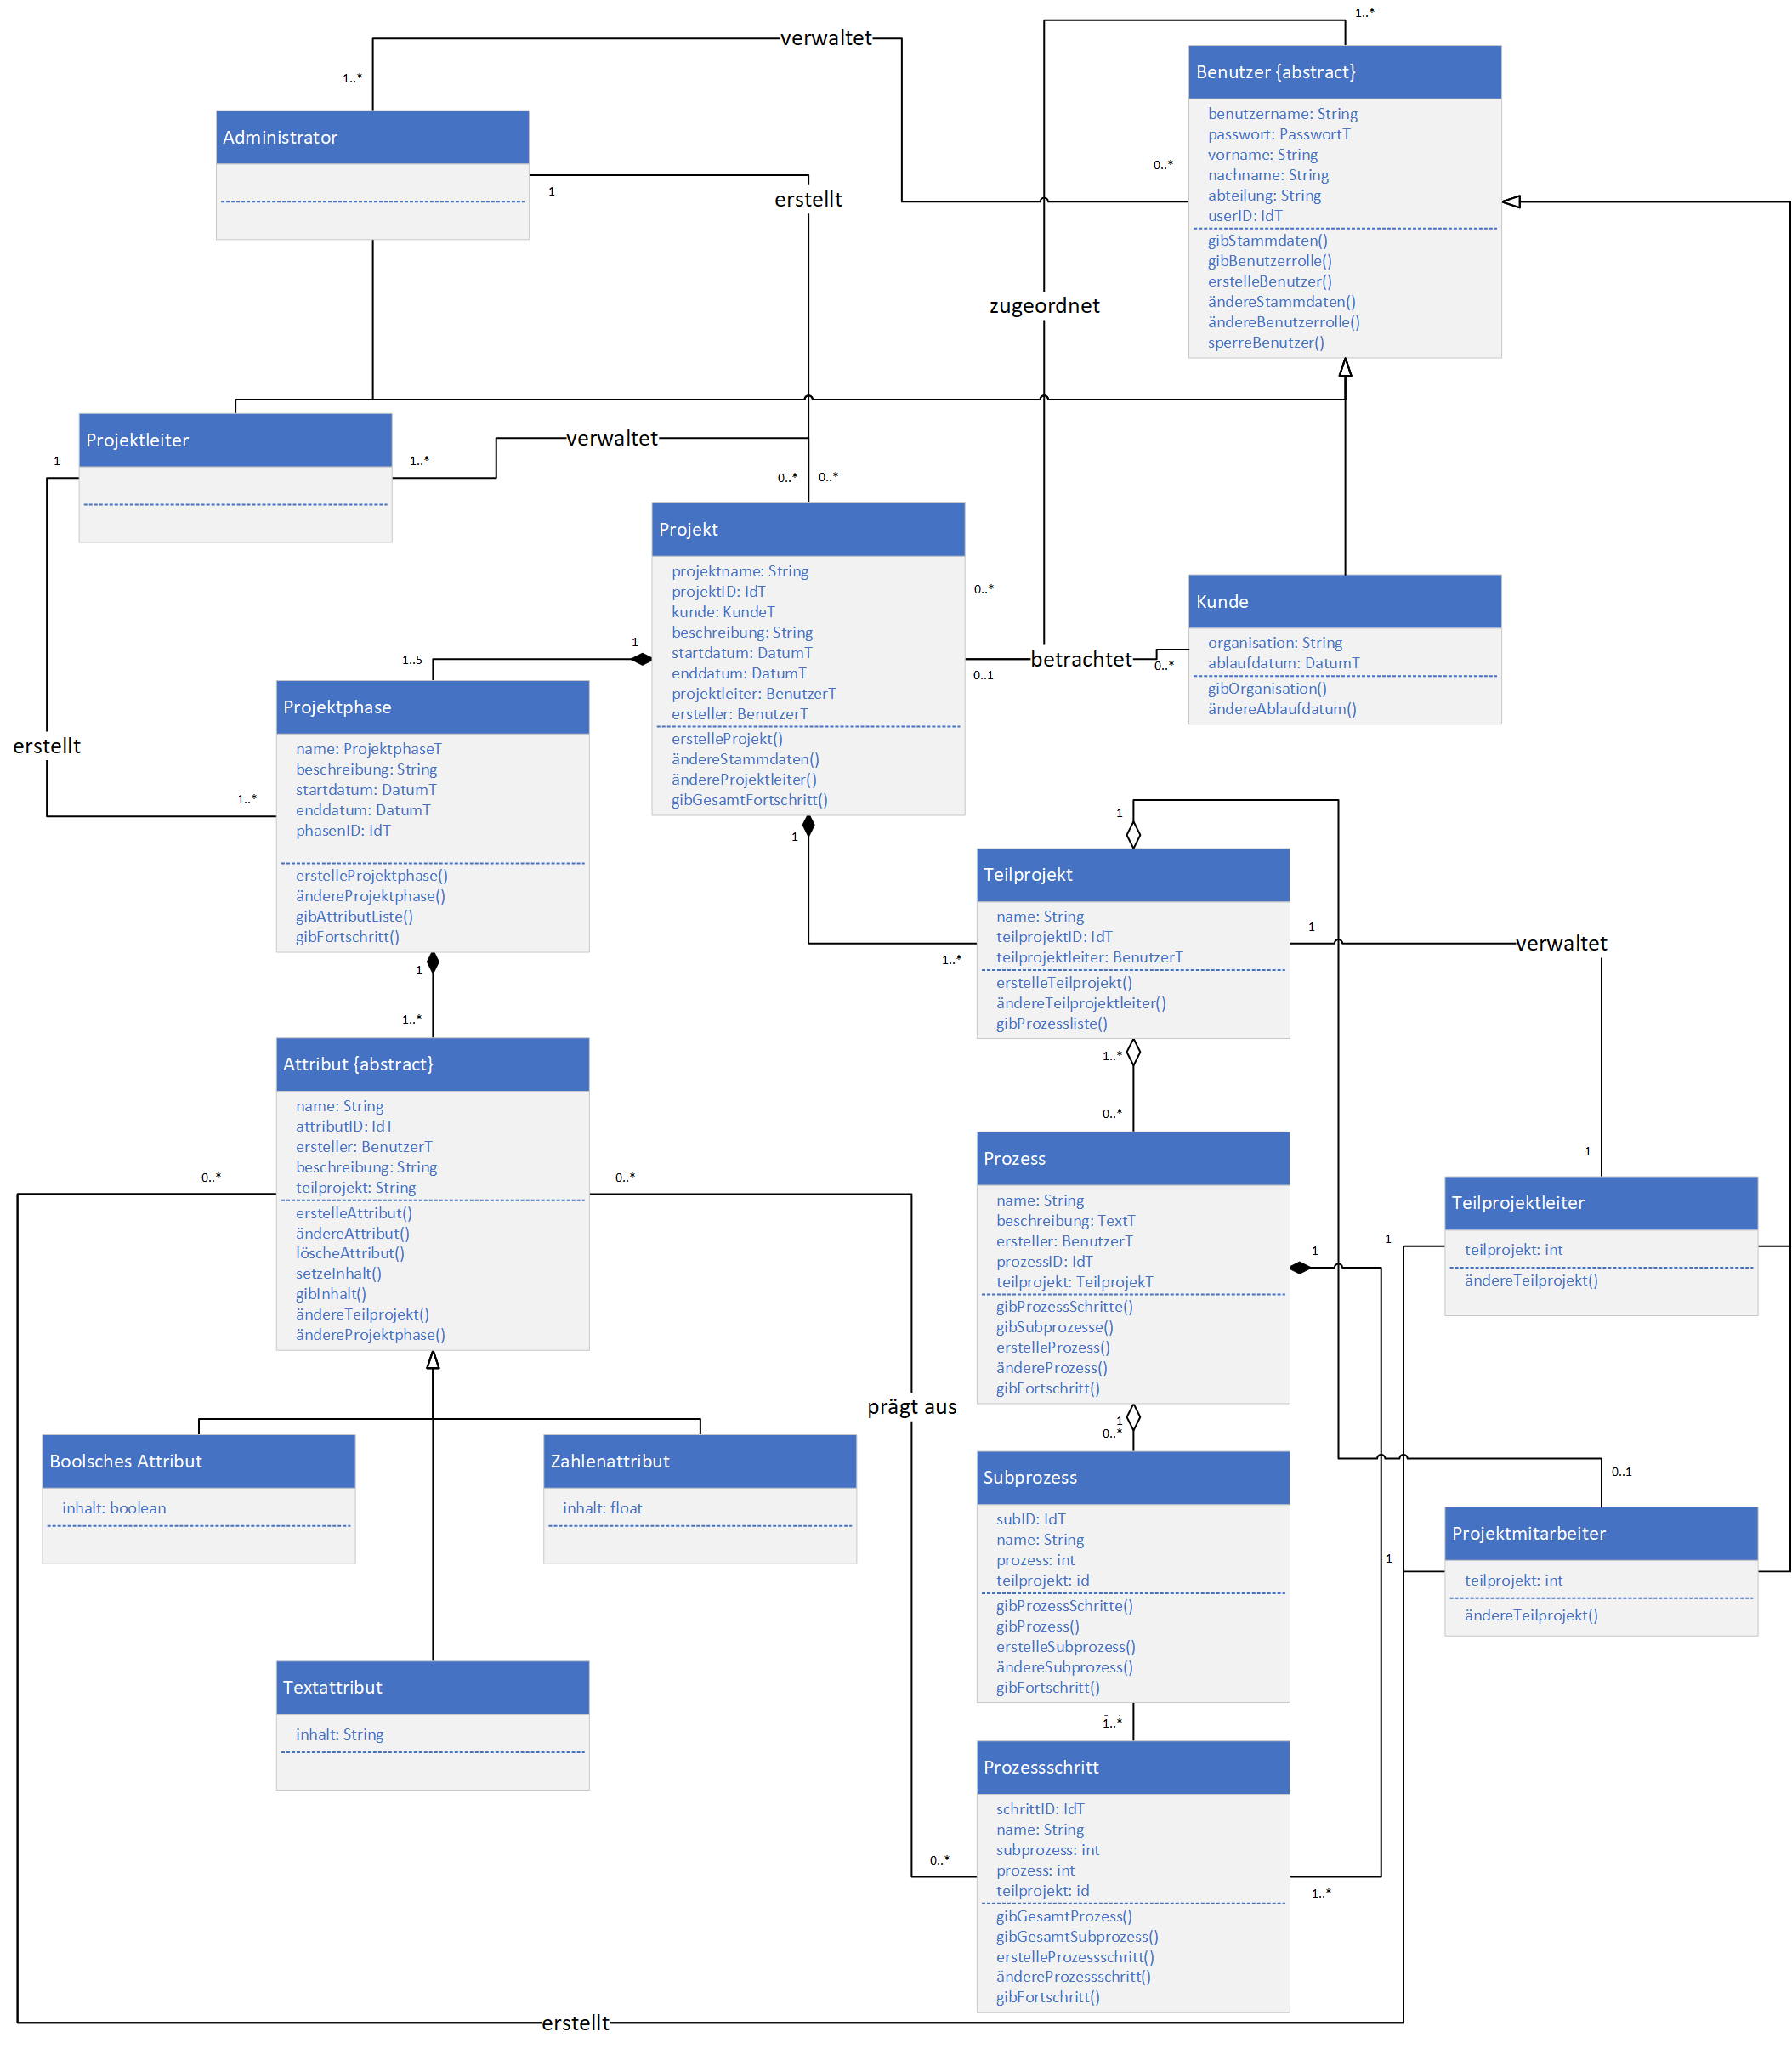
\includegraphics[scale=0.45]{./Bilder/Klassendiagramm.png}
    \caption[Erweitertes Klassendiagramm]{Erweitertes Klassendiagramm}
    \label{fig:Klassendiagramm}
\end{figure}
\emph{Zur verbesserten Anschauung ist das Diagramm ebenfalls im Verzeichnis ./Bilder/Klassendiagramm.png dieser Arbeit abgelegt.}

\newpage
\subsection{Paketdiagramm}
Die nachfolgende Abbildung zeigt die Bündelung der ermittelten Klassen des Business Transformation Trackers zu vier Paketen in einem Paketdiagramm.\\
\begin{figure}[h!]
    \centering
    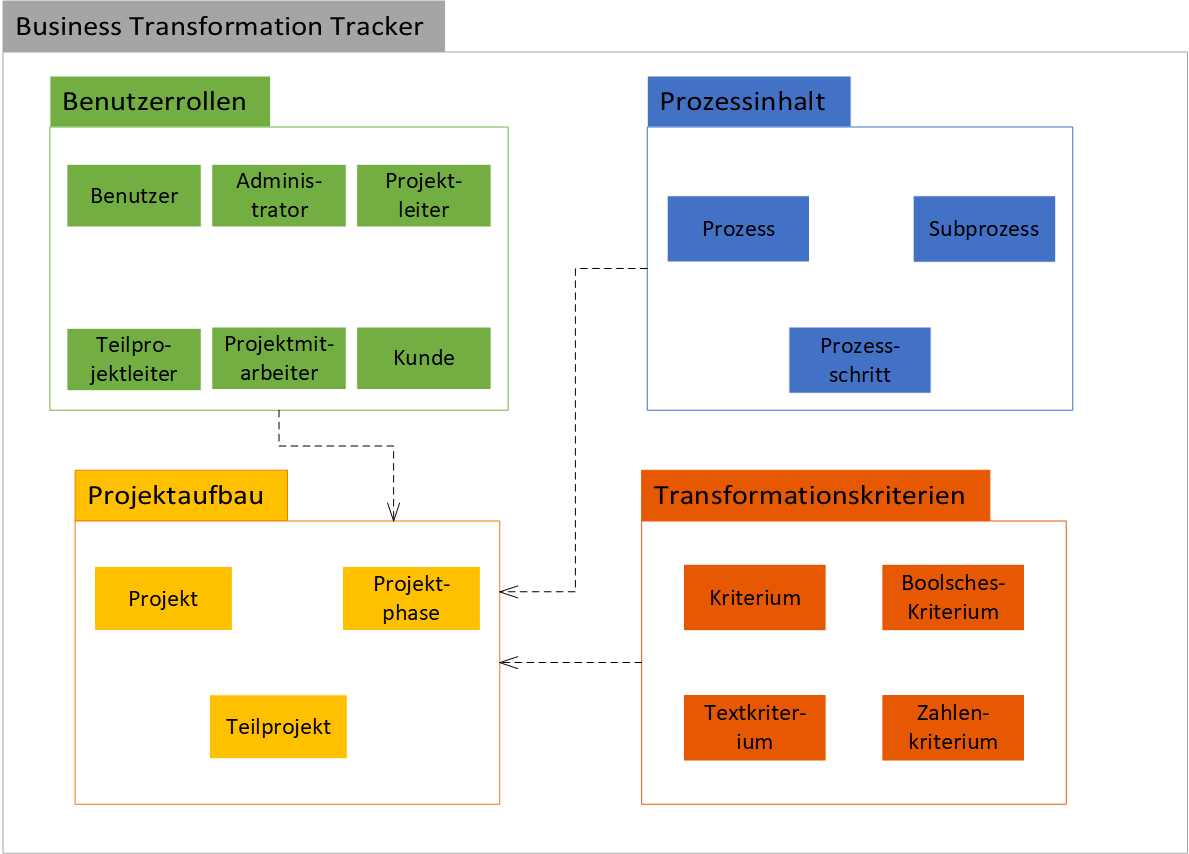
\includegraphics[scale=0.8]{./Bilder/Paketdiagramm.png}
    \caption[Paketdiagramm]{Paketdiagramm}
    \label{fig:Paketdiagramm}
\end{figure}
\\Die ermittelten Pakete sind \glqq{}Benuterrollen\grqq{}, \glqq{}Projektaufbau\grqq{}, \glqq{}Prozessinhalt\grqq{} und \glqq{}Transformationskriterien\grqq{}. 
\vspace{1em}
\\Das Paket \underline{Benutzerrollen} enthält die Klassen \emph{Benuter, Administrator, Projektleiter, Teilprojektleiter, Projektmitarbeiter und Kunde}. Diese Klassen werden für den Aufbau der Berechtigungen und der Rollen benötigt werden. 
\vspace{1em}
\\In dem Paket \underline{Projektaufbau} befinden sich die Klassen \emph{Projekt, Projektphase und Teilprojekt}, die im System für den Aufbau des Projektes zuständig sind. 
\vspace{1em}
\\In dem Paket \underline{Prozessinhalt} befinden sich die Klassen \emph{Prozess, Subprozess und Prozessschritt}, die in der direkten Interaktion mit dem Anwender stehen. Mit ihnen werden die Geschäftsprozesse im System erfasst, indem diese nach Prozess, Subprozess und Prozessschritt aufgespalten werden. 
\vspace{1em}
\\Das Paket \underline{Transformationskriterien} enthält die Klassen \emph{Kriterium, BoolschesKriterium, Textkriterium und Zahlenkriterium}, die für die Ausprägung der Fortschrittserfassung der Geschäfts-prozesse benötigt werden.
\vspace{1em}
\\Es bestehen Abhängigkeiten zwischen den Paketen \underline{Projektaufbau} und \underline{Prozessinhalt}; \underline{Prozessinhalt} und \underline{Transformationskriterien}; \underline{Benutzerrollen} und \underline{Projektaufbau} sowie zwischen \underline{Projektaufbau} und \underline{Transformationskriterien}. In allen fällen ist das Paket \underline{Projektaufbau} das unabhängigste, da eine Änderung hier sich mit großer Wahrscheinlichkeit auch auf die anderen Pakete auswirkt, jedoch nicht umgekehrt.
\vspace{1em}
\\\emph{Zur verbesserten Anschauung ist das Diagramm ebenfalls im Verzeichnis ./Bilder/Paketdiagramm.png dieser Arbeit abgelegt.}












\begin{comment}
%überarbeiten, an neues Buch anpassen
%Anforderungen --> Anforderungsspezifikation --> Fachliche Lösung
In dem nun folgendem Kapitel wird die Anforderungsanalyse behandelt. Orientiert wird sich dazu an dem Vorgehensmodell von Helmut Balzert, das ausführlich in dem Modul BIS-134 Anforderungsanalyse des Studiengangs Wirtschaftsinformatik der Hochschule Hannover behandelt wurde.\\Die Anforderungsanalyse ist einer der ersten Schritte im Softwareentwicklungsprozess und hat zum Ziel die Anforderungen zu ermitteln, die das System, in diesem Fall der Business Transformation Tracker, leisten soll, sowie diese zu definieren. Dadurch soll eine größtmögliche Abdeckung der gestellten Anforderungen erreicht werden und Unstimmigkeiten mit dem Kunden, bzw. dem Auftraggeber, in Bezug auf Funktion und Umfang, vermieden werden. Im Wasserfallmodell nach Balzert ist die Anforderungsanalyse in der Definitionsphase verortert und arbeitet somit mit den Ergebnisobjekten der vorangegangenen Planungsphase. \footcite[Vgl.][S. 100 ff.]{balzert} Die Ergebnisse der Anforderungsanalyse werden dem anschließenden Kapitel, der Konzeption und somit der Entwurfsphase, als Basis dienen.\\
Im Rahmen dieser    Darstellung in UML


\subsection{Ermittlung der Anforderungen}
Im nachfolgendem Kapitel werden die Anforderungen an die Software, die sich aus der Problemstellung und Gesprächen mit dem Auftraggeber ergeben haben, genauer spezifiziert. Im Anschluss folgen dann die zusätzlichen Anforderungen, die sich aus der Umfrage ergeben haben.

\subsubsection{Nichtfunktionale Anforderungen}
%Anforderungen müssen systematisch gewonnen werden von Beteiligten und Betroffenen, sonstige quellen

\subsection{Spezifizierung der Anforderungen}
%Ermittelte Anforderungen müssen spezifiziert werden, unter Berücksichtigung von festgelegten Methoden, Richtlinien, etc.

\subsection{Analyse der Anforderungen}
%Spezifizierte Anforderungen müssen anhand von Richtlinien und Checklisten analysiert werden

\subsection{Modellierung der Anforderungen}
%analysierte und validierte Anforderungen bilden Ausgangspunkt für Modellierung der fachlichen Lösung

\subsection{Verifikation der Anforderungen}

\subsection{Wahl der Entwicklungsplattform}
warum java, nicht web, nicht abap, nicht etc..
bewertung der it sicherheit anhand bestimmter kriterien (datenschutz, zugriffssicherheit, bewahrung von geschäftsgeheimnissne), java weil protierung auf allen plattformen (windows, unix, macos) verfügbar

\subsection{Pflichtenheft}
Durch den Auftraggeber wurden folgende Anforderungen gestellt:

\subsection{Use-Cases}
Akteure des IT-Systems definieren
Mitarbeiter: Projektmitarbeiter, Projektleiter, Teilprojektleiter
Usecase 1:
Der Projektleiter möchte ein neues Projekt anlegen und die Mitarbeiter zuordnen

Usecase 2:
Der Teilprojektleiter öffnet ein vorhandenes Projekt und fügt erfasst die Prozesse und Subprozesse

Usecase 3:
Ein Projektmitarbeiter möchte den aktuellen Fortschritt in einem Subprozess erfassen.

\subsection{Umgebung}
\subsection{Schnittstellen}

%Methodik
\begin{comment}
    %Methodik
    --> Wasserfallmodell nach Helmut Balzert(1995), S.100 ff.

    Anwendungsfälle
    Geschäftsprozessdiagramm, Aktivitätsdiagramm (Folie 94)
    Anwendungsfalldiagramm, -schablone
    Klassendiagramme --> Beziehungen --> Detailliertes Klassendiagramme
    Attribute Spezifizieren (exemplarisch), Operationen
    Sequenzdiagramm

    Pflichtenheft (genaue spezifizierung) 
    Verfeinerung des Lastenheftes
    Verbale Beschreibung dessen, was das System leisten soll (Auftraggebersicht)
    Dient i. a. als vertragliche Beschreibung des Lieferumfangs
    Einstiegsdokument für alle, die das System später pflegen und warten sollen
    Grundlage für die Erstellung des Produkt-Modells

    Ziel
    •Präzise Festlegung, WAS das System leisten soll (aus Sicht des Auftraggebers)
    Anforderungsanalyse
    •Ermittlung und Beschreibung der Anforderungen des Auftraggebers an ein IT-System
    •Bestimmung dessen, WAS das System leisten soll
    •Erstellen eines logischen Modells

\end{comment}